\documentclass[12pt,letterpaper]{article}
\usepackage[utf8]{inputenc}
\usepackage[spanish]{babel}
\usepackage{graphicx}
\usepackage[left=2cm,right=2cm,top=2cm,bottom=2cm]{geometry}
\usepackage{graphicx} % figuras
% \usepackage{subfigure} % subfiguras
\usepackage{float} % para usar [H]
\usepackage{amsmath}
%\usepackage{txfonts}
\usepackage{stackrel} 
\usepackage{multirow}
\usepackage{enumerate} % enumerados
\renewcommand{\labelitemi}{$-$}
\renewcommand{\labelitemii}{$\cdot$}
% \author{}
% \title{Caratula}
\begin{document}

% Fancy Header and Footer
% \usepackage{fancyhdr}
% \pagestyle{fancy}
% \cfoot{}
% \rfoot{\thepage}
%

% \usepackage[hidelinks]{hyperref} % CREA HYPERVINCULOS EN INDICE

% \author{}
\title{Caratula}

\begin{titlepage}
\begin{center}
\large{UNIVERSIDAD PRIVADA-DE-TACNA}\\
\vspace*{-0.025in}
\begin{figure}[htb]
\begin{center}

\includegraphics[width=8cm]{./Imagenes/logo}
\end{center}
\end{figure}
\vspace*{0.15in}
INGENIERIA DE SISTEMAS  \\
\vspace*{0.5in}
\begin{large}
TITULO:\\
\end{large}
\vspace*{0.1in}
\begin{Large}
\textbf{Sistema de Recomendación de Libros de Biblioteca} \\
\end{Large}
\vspace*{0.3in}
\begin{Large}
\textbf{CURSO:} \\
\end{Large}
\vspace*{0.1in}
\begin{large}
INTELIGENCIA DE NEGOCIOS\\
\end{large}
\vspace*{0.3in}
\begin{Large}
\textbf{DOCENTE(ING):} \\
\end{Large}
\vspace*{0.1in}
\begin{large}
 Patrick Cuadros Quiroga\\
\end{large}
\vspace*{0.2in}
\vspace*{0.1in}
\begin{large}
Integrantes: \\
\begin{flushleft}
Acosta Ortiz, Orlando Antonio                  \hfill	(2015052775) \\
Zegarra Reyes, Roberto  		            \hfill 	(2010036175) \\
Catari Cabrera, Yofer Nain 		\hfill 	(2017059289) \\
Mamani Maquera, Jorge Luis                   \hfill 	(2016055236) \\
Rivas Rios, Marko Antonio                       \hfill 	(2016054461) \\
Cruz Escalante, Richard Manuel             \hfill 	(2013047247) \\
\end{flushleft}
\end{large}
\end{center}
\end{titlepage}




\tableofcontents % INDICE
\thispagestyle{empty} % INDICE SIN NUMERO
\newpage
\setcounter{page}{1} % REINICIAR CONTADOR DE PAGINAS DESPUES DEL INDICE

\section{RESUMEN} 


\section{INTRODUCCION} 


Con la finalidad de tener una biblioteca con información actualizada y brindar información rápida diferentes medios bibliográficos de la biblioteca, además de poder realizar reservaciones desde el sistema.
\\
Este sistema será de mucha utilidad para ubicar un libro y otros medios de la biblioteca rápidamente, nos facilitará conocer el status de los libros y préstamos, la adquisición de nuevos libros y los procesos técnicos por ejemplo catalogación y clasificación de los ejemplares.
\\

Los beneficios sociales que un proyecto serio y estructurado de un sistema para la administración de Biblioteca, en el cual se involucren diferentes sectores de un ente académico, privado, de carácter estatal o del gobierno, son simples y fácilmente demostrables.\\

La finalidad principal de un proyecto de este tipo es la generación, administración y disposición de conocimiento para una comunidad determinada.
Los beneficios académicos que recibirá la institución es automatizar estos procesos con un sistema de Inventario y préstamos de libros haciendo la tarea más sencilla para los estudiantes y el administrador de la misma.\\
Con la implementación de esta herramienta se obtendrá la información al instante de los libros, revista, editoriales entre otros. Se podrá obtener una lista de todos los libros en stock, editoriales, etc., y buscar en cualquier momento en base a varios reglas de filtrado. Se podrá organizar la biblioteca por editoriales, autores entre otros.

\section{MARCO TEORICO} 


\subsection{Python}
	
Python es un lenguaje sencillo y rápido de aprender. Su sintaxis es parecida a escribir cualquier texto en inglés, pero con la potencia de sus principales competidores en el BackEnd.
Es un placer de leer y redactar. Python predica que un código debe ser escrito por humanos para humanos. Después de todo lo que programas va a ser leído por ti y por el resto del equipo. Si escribes para máquinas, solo te entenderán máquinas.
\\
Además, viene con “Pilas incluidas”. Eso quiere decir que posee su propio gestor de paquetes, sin necesidad de instalar aplicaciones externas. Simplificando tareas de instalación o actualización.
\\
Otro punto a su favor es que no necesita un ecosistema para ejecutarse, como puede ser Xampp, Vangrant, Docker… Python solo requieres Python. Lanzando un comando en el terminal estará ejecutándose su propio servidor Web, consiguiendo que su puesta en producción sea sorprendentemente rápida.
Y por si fuera poco, es el segundo lenguajes que mejor esta pagado por las empresas. Por detrás de Ruby.

\subsection{Google Colab: Python y Machine Learning en la nube}
En este veremos qué es y cómo utilizar Google Colab, la herramienta de Google en la nube para ejecutar código Python y crear modelos de Machine Learning a través de la nube de Google y con la posibilidad de hacer uso de sus GPU . Sí, has leído bien: con sus GPU y en la nube.


		
\subsection{Frameworks Web}

Entre sus numerosos y fantásticos Frameworks, nos podemos encontrar unas bestias: Django y Flask (que no confundir que el zombie Adobe Flash).
Django sería lo más cercano a Laravel en PHP o Ruby on Rails para Ruby. Un marco de trabajo completo y eficiente para desarrollar Aplicaciones Web de una gran complejidad con un mínimo esfuerzo. Casi cualquier cosa que necesites posiblemente estará integrada.
\\
Para desarrollos altamente personalizados o con unos tiempos cortos, nos encontramos a Flask. Autodenominado microframework, pero con funcionalidades sencillas e inteligentes para construir cualquier sitio que se te pase por la cabeza.
Uno no sustituye al otro. Merece la pena experimentarlos y ver sus diferentes enfoques. 


	
\subsection{Ventajas de programar en Python}
\begin{itemize}	
\item	Simplificado y rápido: Este lenguaje simplifica mucho la programación, es un gran lenguaje para scripting.\\
\item	Elegante y flexible: El lenguaje ofrece muchas facilidades al programador al ser fácilmente legible e interpretable.\\
\item	Programación sana y productiva: Es sencillo de aprender, con una curva de aprendizaje moderada. Es muy fácil comenzar a programar y fomenta la productividad.\\
\item	Ordenado y limpio: es muy legible y sus módulos están bien organizados.\\
\item	Portable: Es un lenguaje muy portable. Podemos usarlo en prácticamente cualquier sistema de la actualidad.\\
\item	Comunidad: Cuenta con un gran número de usuarios. Su comunidad participa activamente en el desarrollo del lenguaje.\\


	

\subsection{Futuro}

Las previsiones son muy buenas. Las versiones son constantes y compatibles con todas las plataforma. Su creador, Guido van Rossum, es denominado como “Benevolente dictador vitalicio” por dejar que la comunidad tomen las decisiones. Tan solo dejó 4 directrices:
\item	Python debería ser fácil, intuitivo y tan potente como sus principales competidores.
\item	El proyecto sería de Código Abierto para que cualquiera pudiera colaborar.
\item	El código escrito en Python sería tan comprensible como cualquier texto en inglés.
\item	Python debería ser apto para las actividades diarias permitiendo la construcción de prototipos en poco tiempo.

\end{itemize}

	
\section{EJEMPLO} 



\subsection{Ejemplos estadisticos}
	
Se utilizo estos ejemplos para desarrollar el sistema de recomendacion de libros.


\begin{center}
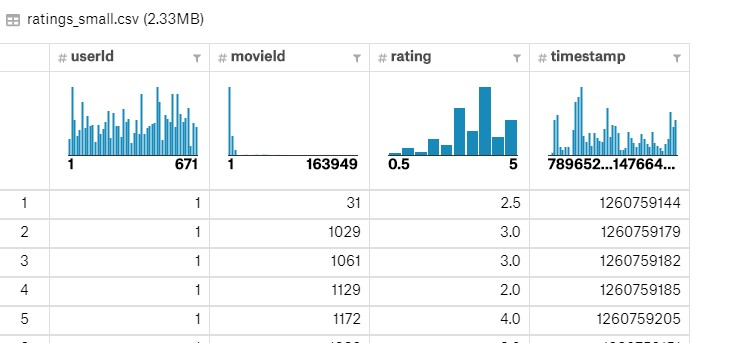
\includegraphics[width=18cm, height=8cm]{./Imagenes/img1.jpg}
\end{center}


\begin{center}
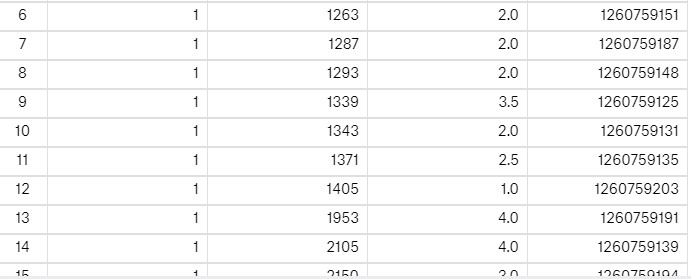
\includegraphics[width=18cm, height=8cm]{./Imagenes/img2.jpg}
\end{center}


\begin{center}
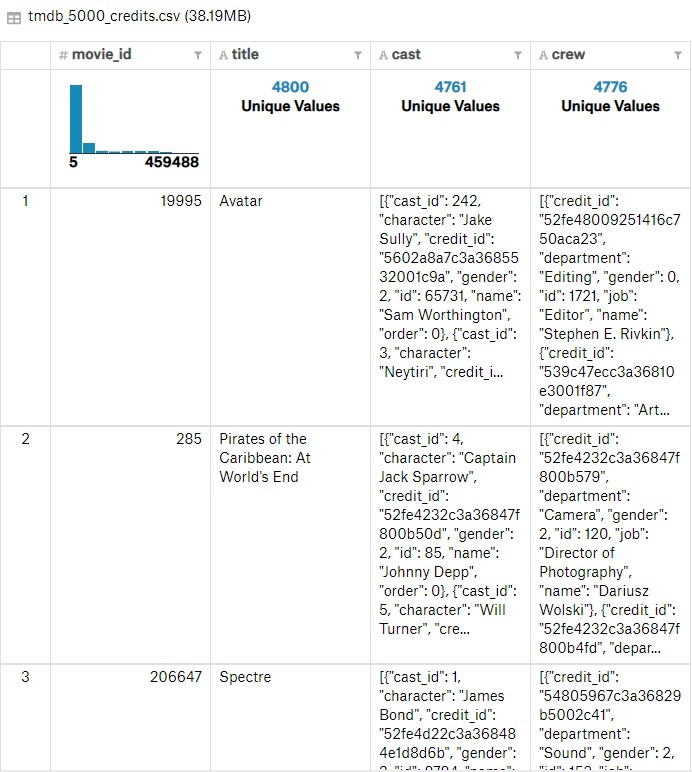
\includegraphics[width=14cm, height=10cm]{./Imagenes/img3.jpg}
\end{center}


\begin{center}
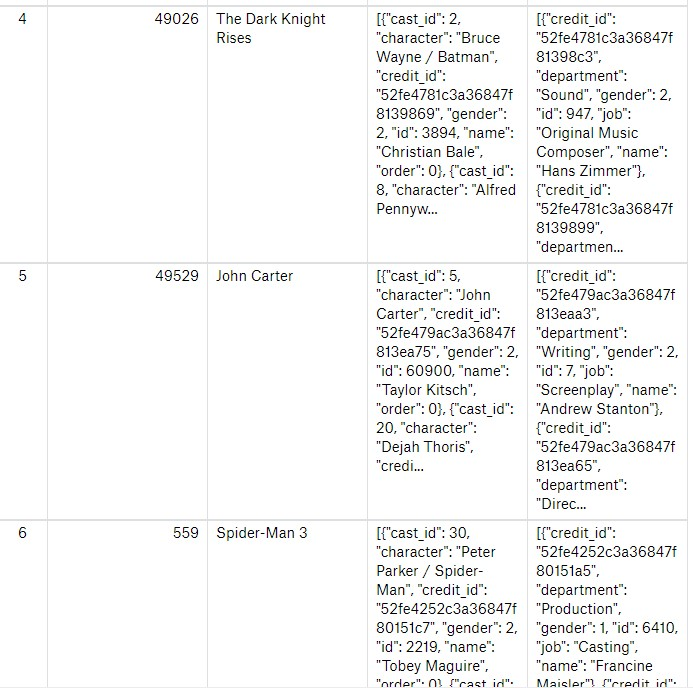
\includegraphics[width=14cm, height=12cm]{./Imagenes/img4.jpg}
\end{center}


\begin{center}
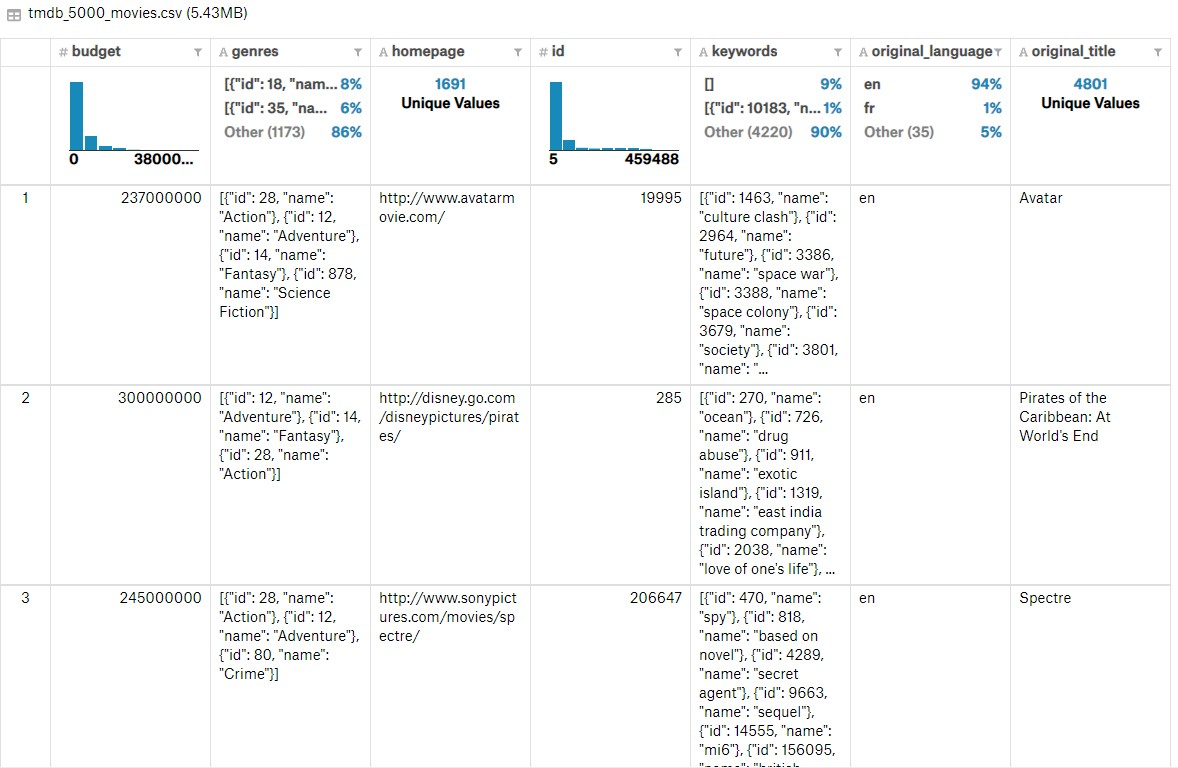
\includegraphics[width=18cm, height=14cm]{./Imagenes/img5.jpg}
\end{center}
\section{ANALISIS} 
\subsection{Datos Estadisticos del sistema de recomendacion de libros}
	
Se utilizo estos ejemplos para desarrollar el sistema de recomendacion de libros.


\begin{center}
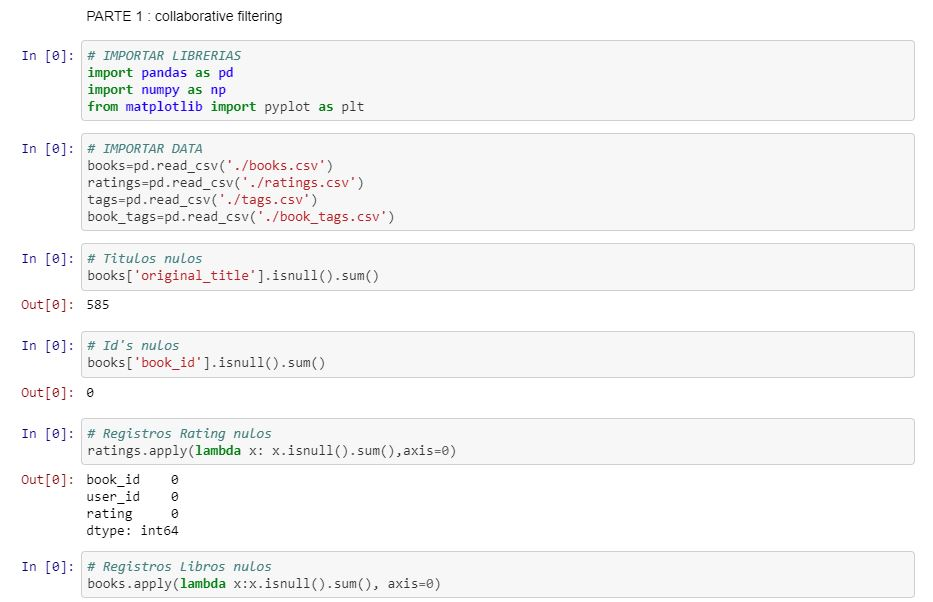
\includegraphics[width=18cm, height=8cm]{./Imagenes/traba1.jpg}
\end{center}


\begin{center}
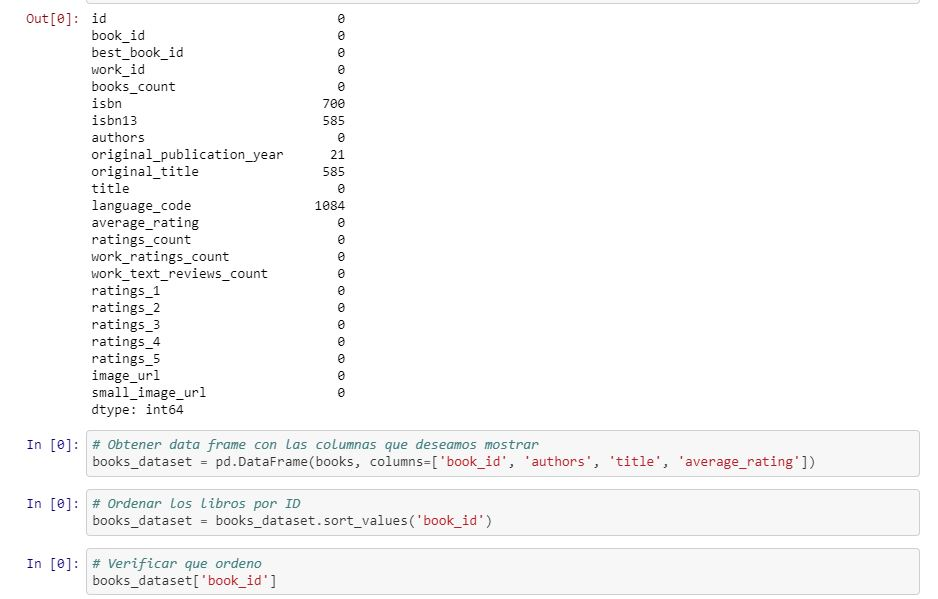
\includegraphics[width=18cm, height=8cm]{./Imagenes/traba2.jpg}
\end{center}


\begin{center}
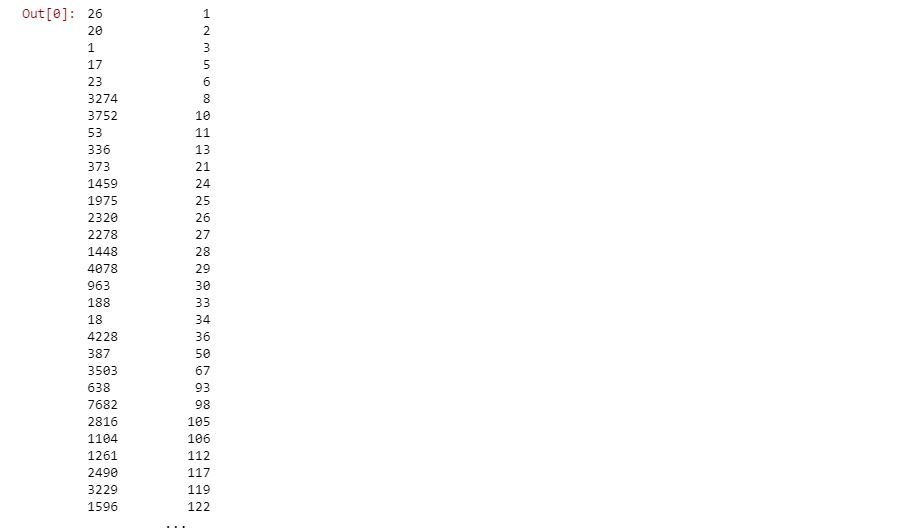
\includegraphics[width=14cm, height=10cm]{./Imagenes/traba3.jpg}
\end{center}


\end{center}


\begin{center}
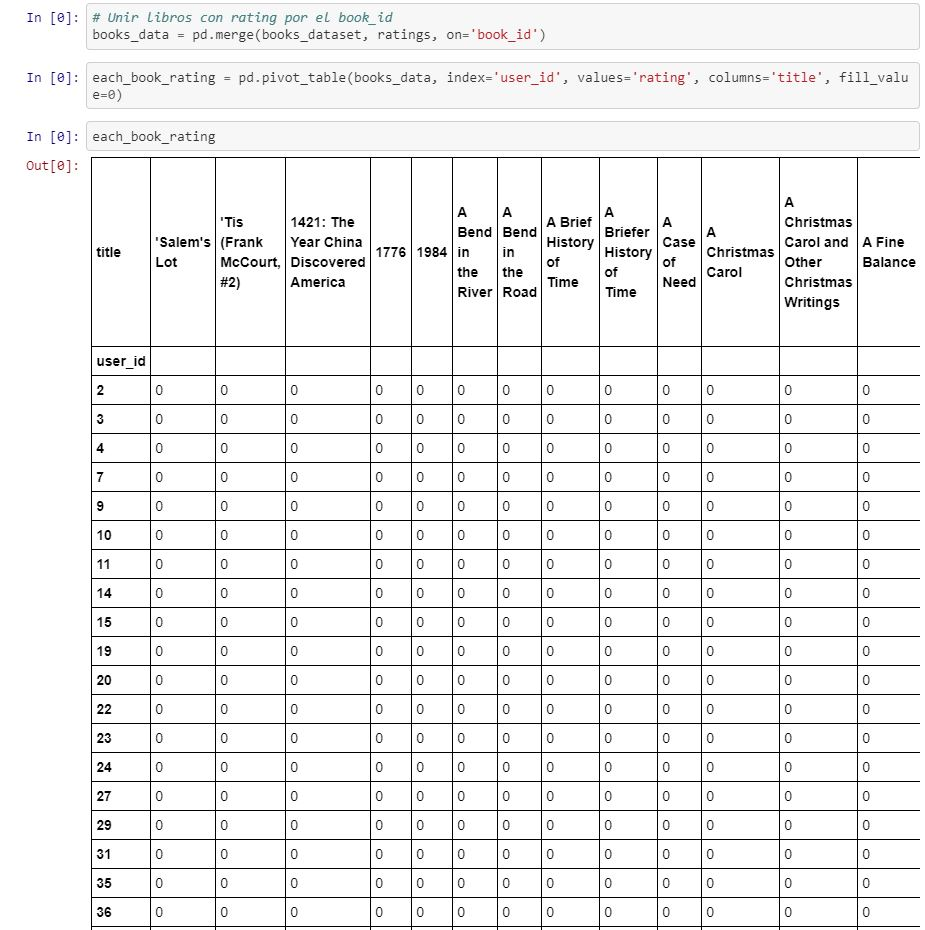
\includegraphics[width=18cm, height=14cm]{./Imagenes/traba5.jpg}
\end{center}

\begin{center}
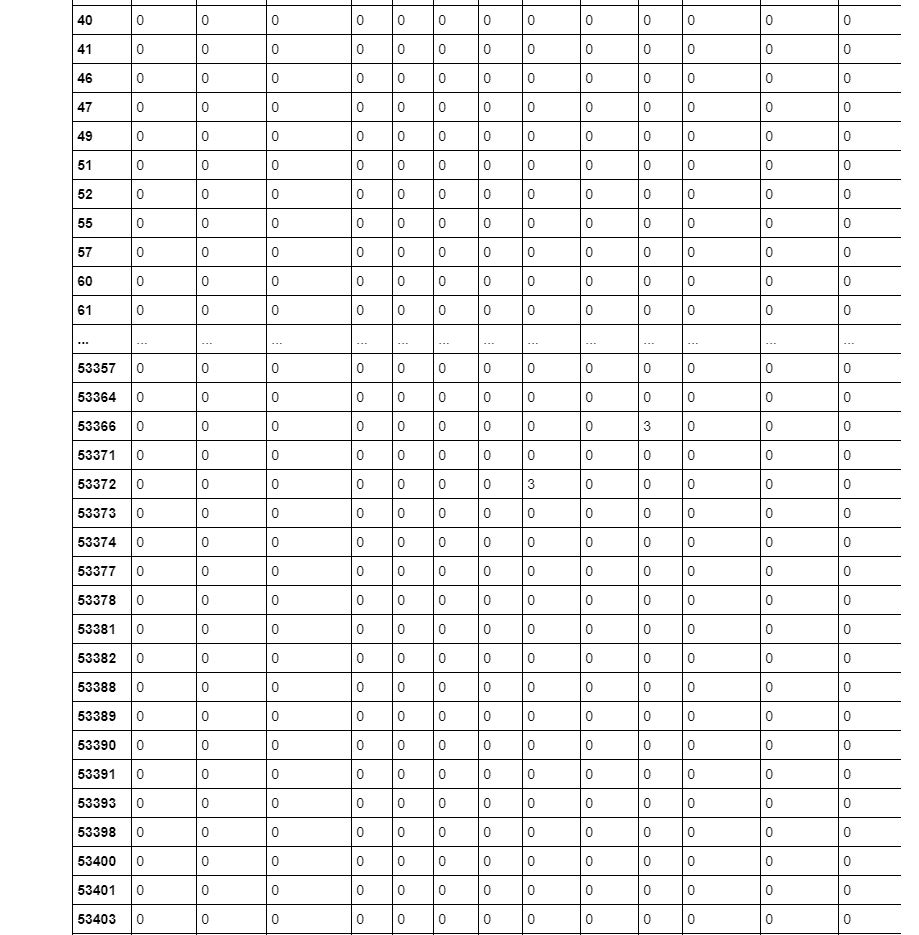
\includegraphics[width=18cm, height=8cm]{./Imagenes/traba6.jpg}
\end{center}


\begin{center}
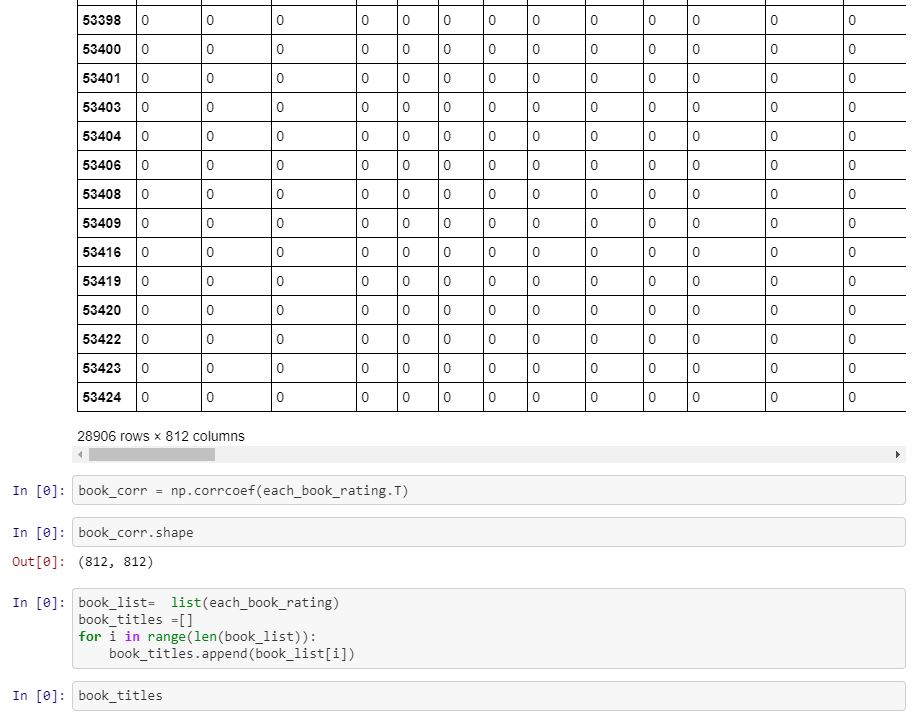
\includegraphics[width=18cm, height=8cm]{./Imagenes/traba7.jpg}
\end{center}


\begin{center}
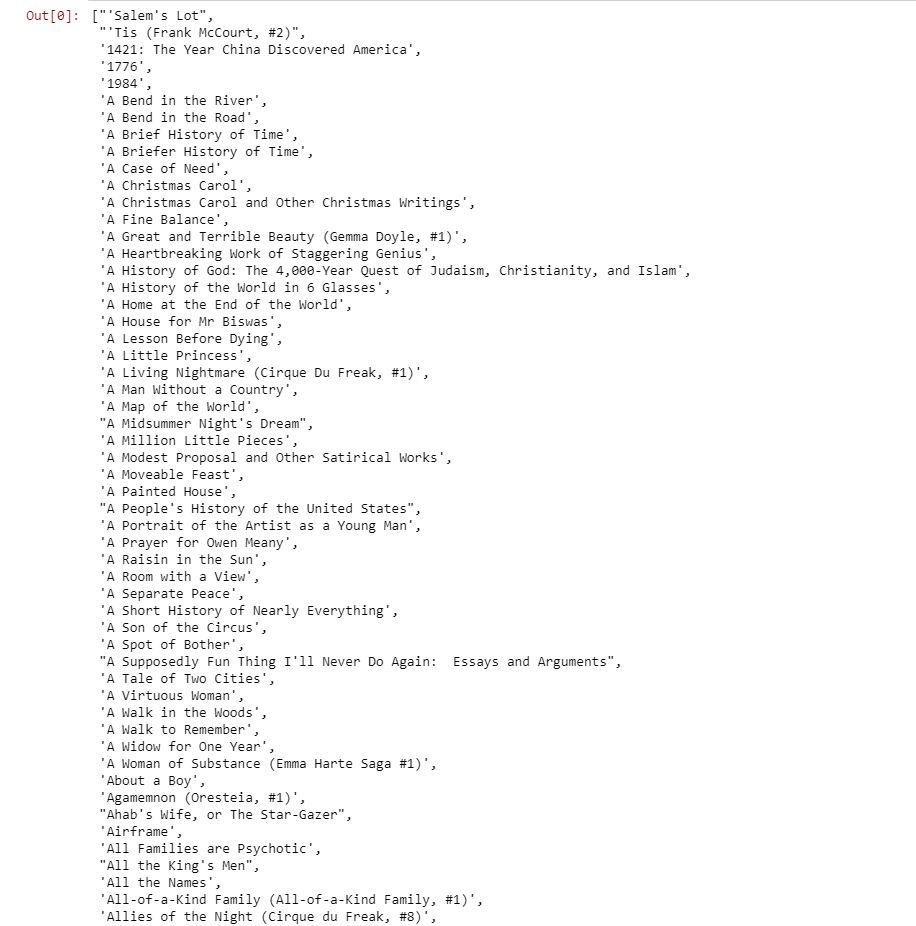
\includegraphics[width=14cm, height=10cm]{./Imagenes/traba8.jpg}
\end{center}


\begin{center}
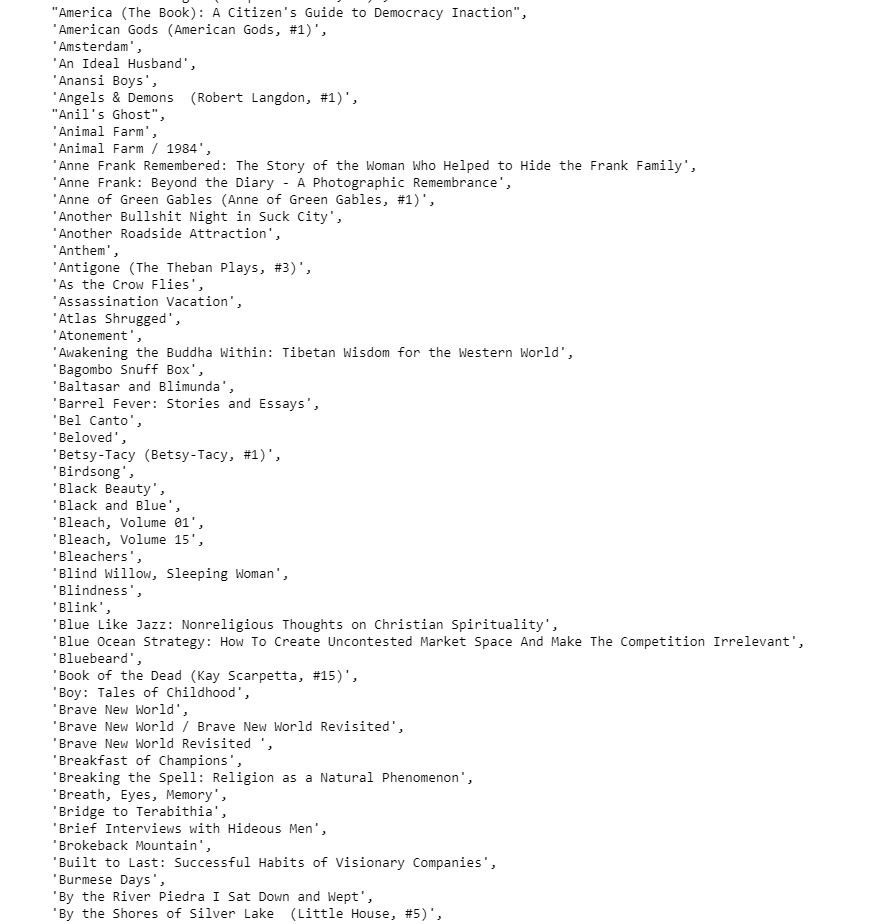
\includegraphics[width=14cm, height=12cm]{./Imagenes/traba9.jpg}
\end{center}


\begin{center}
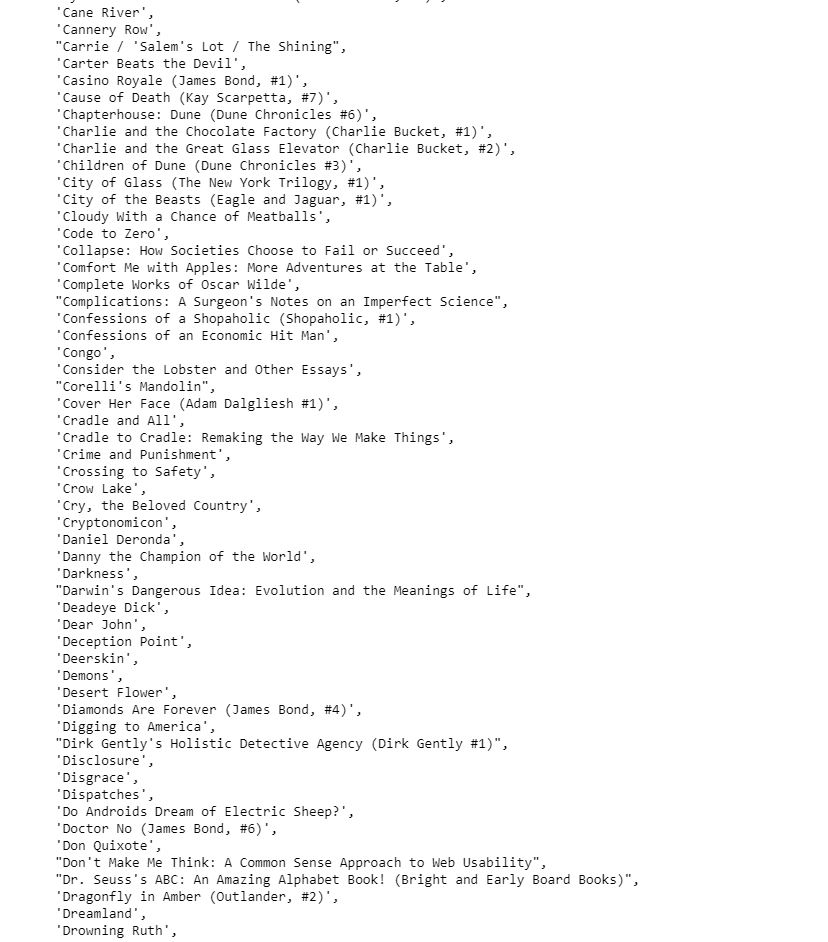
\includegraphics[width=18cm, height=14cm]{./Imagenes/traba10.jpg}
\end{center}

\begin{center}
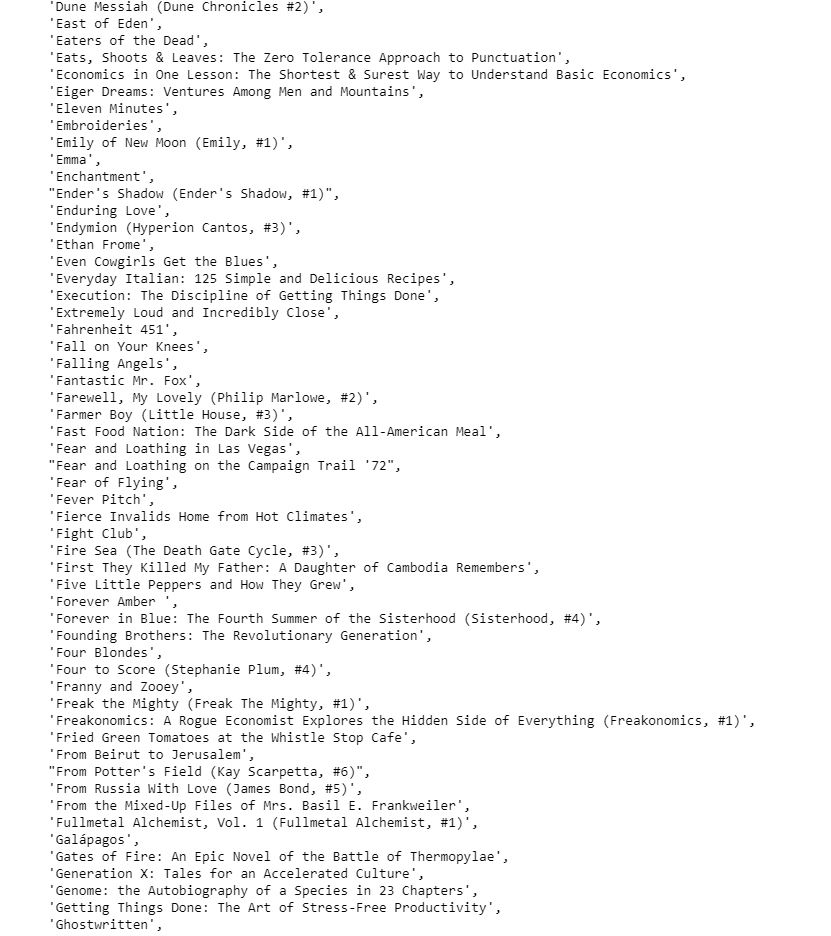
\includegraphics[width=18cm, height=8cm]{./Imagenes/traba11.jpg}
\end{center}


\begin{center}
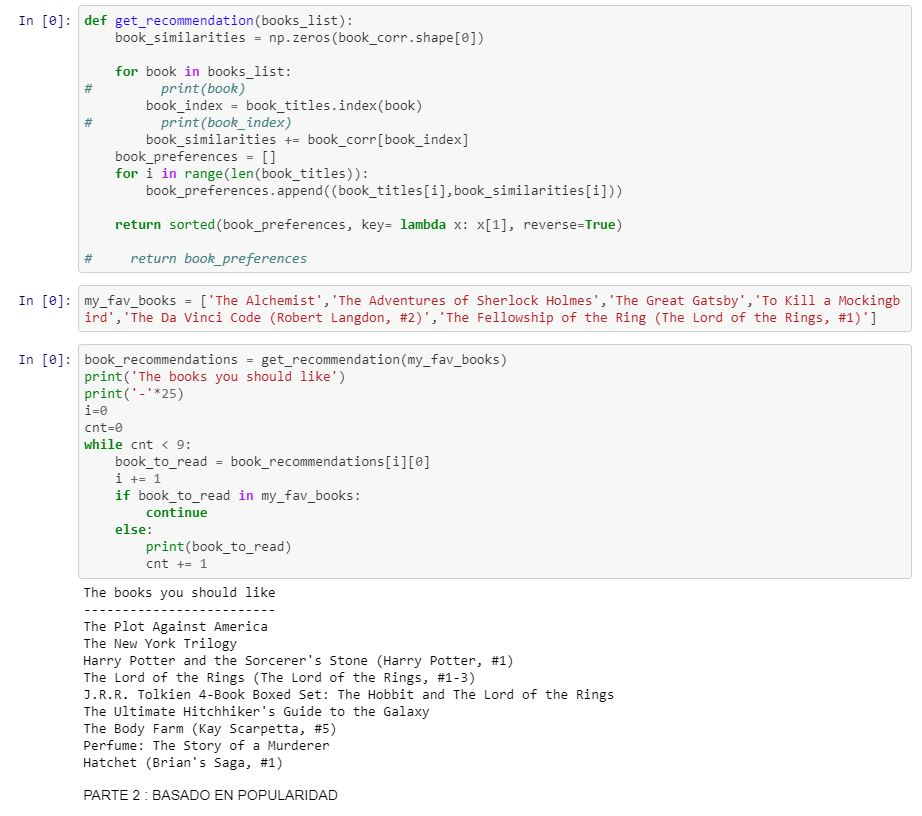
\includegraphics[width=18cm, height=8cm]{./Imagenes/traba12.jpg}
\end{center}


\begin{center}
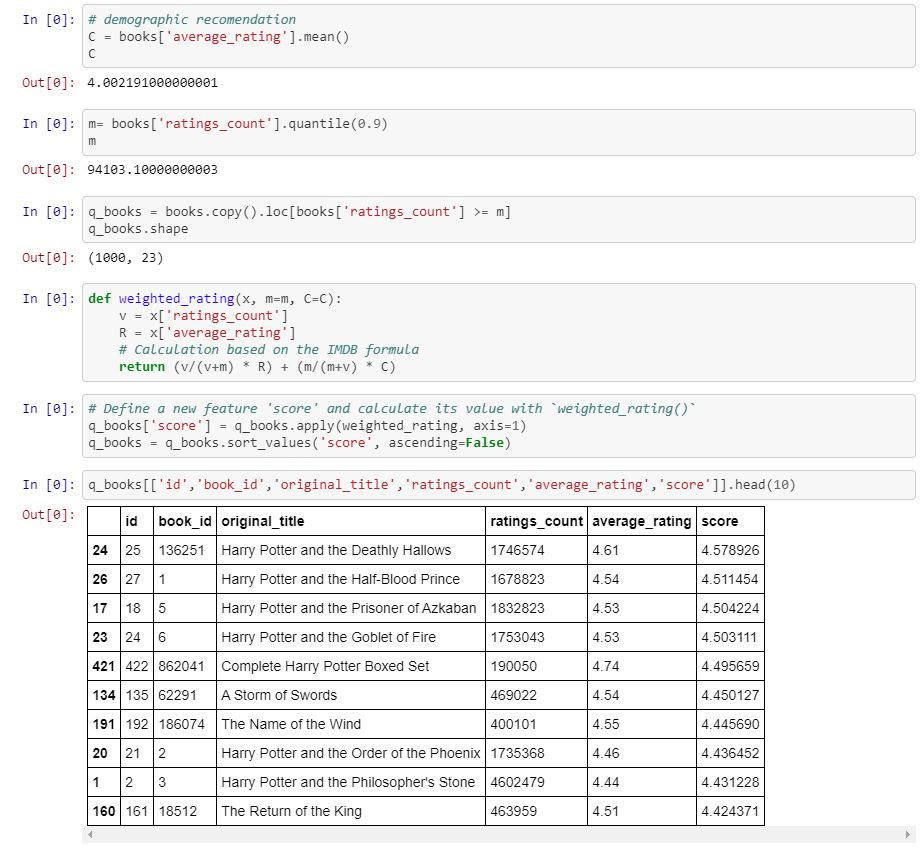
\includegraphics[width=14cm, height=10cm]{./Imagenes/traba13.jpg}
\end{center}


\begin{center}
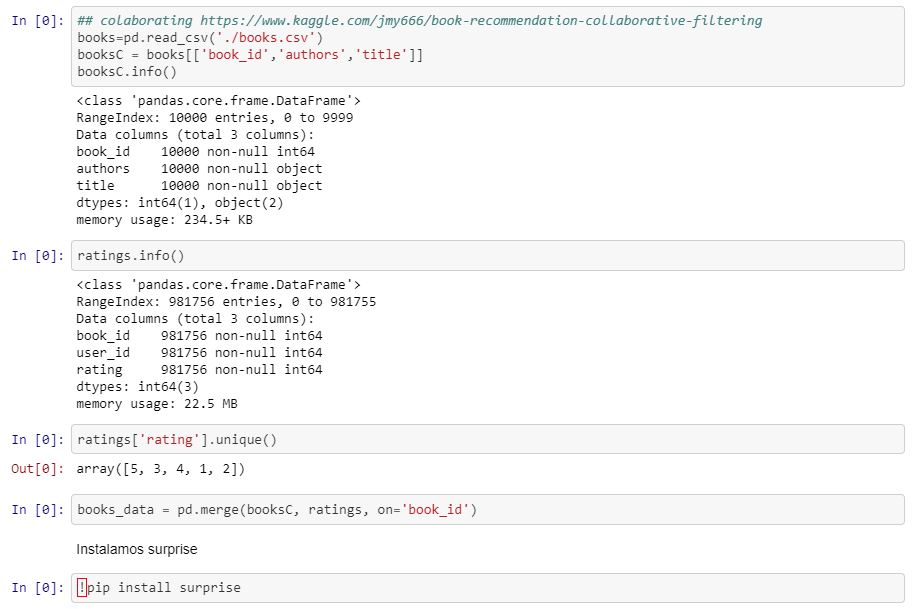
\includegraphics[width=14cm, height=12cm]{./Imagenes/traba14.jpg}
\end{center}


\begin{center}
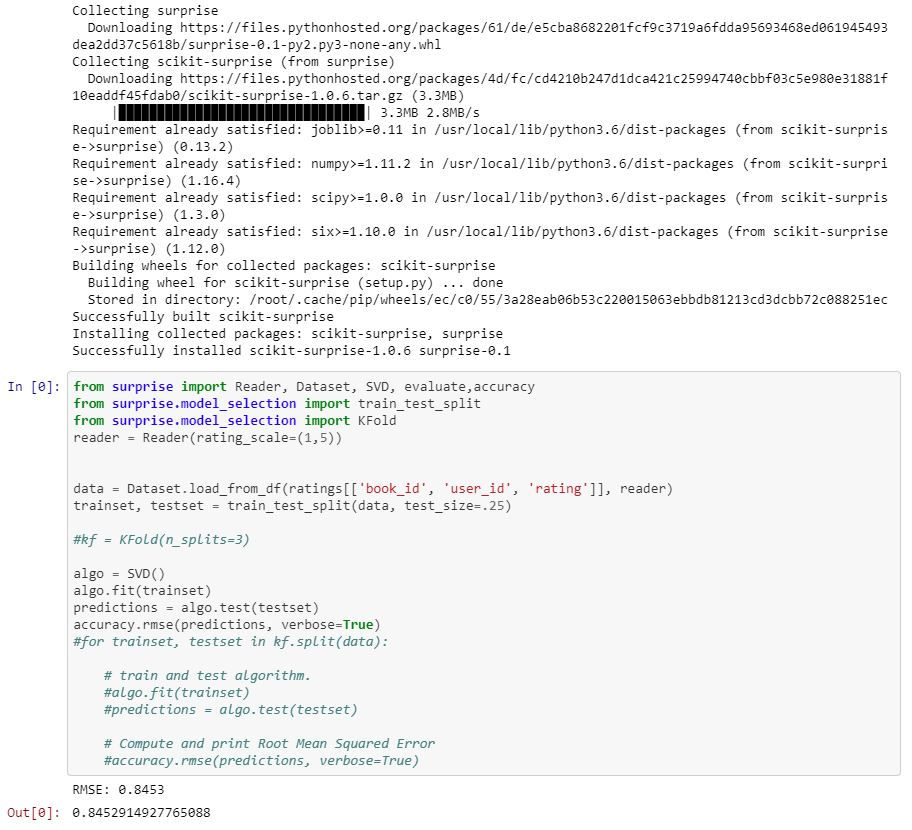
\includegraphics[width=18cm, height=14cm]{./Imagenes/traba15.jpg}
\end{center}

\begin{center}
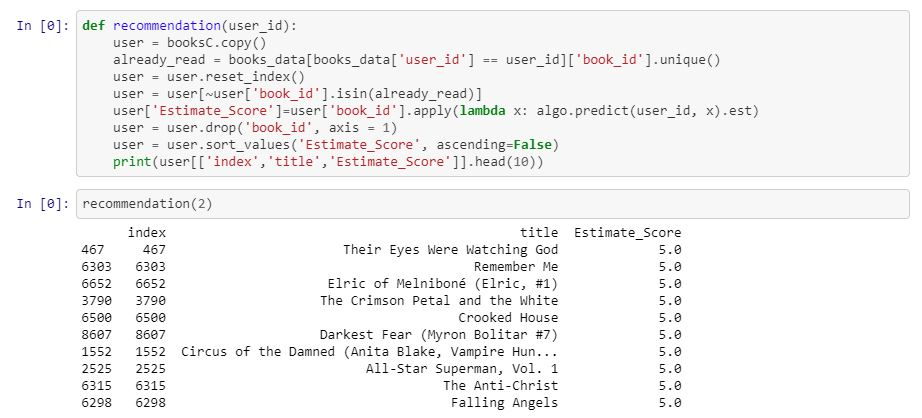
\includegraphics[width=18cm, height=14cm]{./Imagenes/traba16.jpg}
\end{center}
\section{CONCLUSIONES} 


Hemos visto que tenem


\section{BIBLIOGRAFIA} 

\begin{itemize}
\item https://dockertips.com/volumenes
\item https://cerebro-digital.com/panel/knowledgebase/64/ExportarorImportar-contenedor-de-Docker-via-archivo-TAR.html
\item  https://www.docker.com/
\item https://www.campusmvp.es/recursos/post/los-beneficios-de-utilizar-docker-y-contenedores-a-la-hora-de-programar.aspx
\item https://www.colap.io/
\item  https://www.aprendemachinelearning.com/machine-learning-en-la-nube-google-colaboratory-con-gpu/

\end{itemize}
\end{document}
